\documentclass[a4paper,12pt]{article}
\usepackage{amssymb}
\usepackage{geometry}
\usepackage{graphicx}
\usepackage{colortbl}

\geometry{margin=1in}



\begin{document}

Dustin Kane

CMSI 370-01

September 24, 2015

\begin{center}
\section*{Assignment 0924: Usability Study}
\subsection*{Comparing Google Drive and Microsoft OneDrive}
\end{center}

\section{Introduction}

Cloud services are ubiquitous these days. People now have much of the software they use everyday available to them wherever they have internet access. A key component of this cloud-based lifestyle is cloud file hosting. Files are an important part of internet use, so it's only natural that files play an important role in the cloud-computing shift. There are a variety of file-hosting cloud services, and many offer similar features. But two cloud file-hosting services are notable because they provide robust file editing utilities. These services are Google Drive by Google and OneDrive by Microsoft. 

Google Drive began as Google's competitor to Dropbox (perhaps the most well-known cloud-based file-hosting service), offering very similar features. But Google soon married Drive with Google Docs, software that is synonymous with online file editing, under the Google Drive branding.

Microsoft's OneDrive platform was also created as an alternative to Dropbox, one that supposedly integrates well with the Windows ecosystem. But one of OneDrive's key strengths is its integration with Microsoft Office. OneDrive has in-browser versions of Microsoft Word, Excel, and Powerpoint, each of which has a desktop client that is the undisputed leader in its area. These in-browser versions are almost identical to their desktop counterparts and support a surprisingly robust feature set.

Google Docs is the leader in online word processing, whereas Microsoft Word is the leader in offline word processing (and has been for decades). Both are integrated into an online file-hosting platform. Our goal was to see which software provided an interface that was most effective at creating, sharing, and collaborating on documents, as well as providing support for version control.

\section{Usability Metrics}

\subsection{Our Focus}
Our goal was to find which online file-hosting and editing software was the most usable. We chose to focus on four key features that represent a wide spectrum of use cases: creating and editing a document, sharing the document with another person, collaborating on that document with another person using comments, and reverting to previous version of the file. The first was a natural choice: no feature of the editing software is usable unless the user can create and edit files. The second hits file sharing: a key benefit of using cloud services. The third expands on the sharing concept to look at tools used for collaborating on a single document between multiple people. The final feature is a lesser-known and more complex feature that is incredibly powerful if used properly.

\subsection{Our Method}

We developed three tasks to be performed in both clients by our test subjects. First, the user had to create a new document, name it ``cats'', type ``dog'' for the body, and then share the document with the email address ``kcgotfre@gmail.com''. For the second task, the user had to highlight the word ``dog'' from the first task and leave a comment on it that said ``woof woof''. We explained to the users first what a comment was and how it was meant to leave notes to collaborators without actually editing the document. For the last task, we had created a separate document that we had edited multiple times and we asked the user to revert it to any previous version. For each of these tasks we recorded from the time they began to the time they hit the last necessary button to complete the task. We also counted the number of errors each user made in each task. We had them do all three tasks for a service together, then switch to the other. The first service we tested for each user was chosen randomly at the start of the test.

We noted which users had used the software before and which had not to better assess learnability vs efficiency. We retested many subjects who had no experience with the software again, this time to test efficiency rather than learnability.

\subsection{Our Metrics}

 We focused on three metrics, $learnability$, $efficiency$, and $errors$. The first, learnability, measures how easy an interface is to figure out. A highly learnable interface should allow a brand new user to easily figure out how to do what he or she wants to do. The second, efficiency, measures how fast someone who is knowledgeable of the software can do tasks they know exactly how to do. If someone knows exactly what to do, the only limiting factors involve the limitations of the user interface. The final metric is errors, which measures how often a user does something with an expectation that isn't met. An interface should make sense and be logical to the user. It should correspond to their mental model of what the system should do, and if it doesn't, it isn't an effective interface.

\subsection{Our Data}

A few notes about the following table. First, certain test subjects are listed twice. This is because some subjects who were new to the software were tested again to test efficiency. A Y in ``XP'' means the user was experienced in that software, an N means they were not. ``E'' is the number of errors that occurred during the test whose time is to the left. ``Create'' represents the time the first task took: creating, editing, and sharing a document. ``Comnt'' is the time the second task took: leaving a comment for a collaborator. ``Revert'' is the time the third task took: reverting the document to an older version.

\begin{table}[h]
\footnotesize
\centering
\begin{tabular}{|c|c|c|c|c|c|c|c|c|c|c|c|c|c|c|}
		\hline
		Tst& \multicolumn{7}{c}{Microsoft OneDrive} & \multicolumn{7}{|c|}{Google Drive} \\
		Sub & XP&Create&E&Comnt&E&Revert&E&XP&Create&E&Comnt&E&Revert&E\\ \hline
Ka1&N&00:35.1&0&00:10.2&0&01:15.1&2&Y&00:13.5&0&00:10.4&0&00:12.0&0\\ \hline
Ka2&N&00:45.1&0&00:51.2&1&00:45.6&0&N&00:30.6&0&00:13.8&0&00:14.9&0\\ \hline
Ka3&N&00:23.2&0&00:26.5&0&00:41.3&0&N&00:19.7&0&00:52.6&1&00:47.2&0\\ \hline
Ka3&Y&00:13.4&0&00:17.8&0&00:24.4&0&Y&00:11.6&0&00:08.7&0&00:19.5&0\\ \hline
Su1&N&01:02.7&0&00:33.0&1&00:47.6&0&Y&00:20.4&0&00:14:5&2&00:24.7&0\\ \hline
Su1&Y&00:20.6&0&00:07.9&0&00:56.5&0&Y&\cellcolor[gray]{0.3}&\cellcolor[gray]{0.3}&\cellcolor[gray]{0.3}&\cellcolor[gray]{0.3}&\cellcolor[gray]{0.3}&\cellcolor[gray]{0.3}\\ \hline
Su2&N&00:59.0&0&00:24.7&0&00:24.8&0&Y&00:32.0&0&00:17.0&0&00:19.1&0\\ \hline
Su2&Y&00:19.3&0&00:14.7&0&00:45.3&0&N&\cellcolor[gray]{0.3}&\cellcolor[gray]{0.3}&\cellcolor[gray]{0.3}&\cellcolor[gray]{0.3}&\cellcolor[gray]{0.3}&\cellcolor[gray]{0.3}\\ \hline
Su3&N&00:34.4&0&00:11.4&0&00:36.6&0&Y&00:16.2&0&00:10.7&0&00:54.4&0\\ \hline
Su4&N&00:44.8&0&00:13.5&0&01:29.2&0&Y&00:17.9&0&00:07.5&0&00:15.7&0\\ \hline
Su4&Y&00:23.5&0&00:07.3&0&00:36.0&0&Y&\cellcolor[gray]{0.3}&\cellcolor[gray]{0.3}&\cellcolor[gray]{0.3}&\cellcolor[gray]{0.3}&\cellcolor[gray]{0.3}&\cellcolor[gray]{0.3}\\ \hline
Su5&N&00:58.8&0&00:10.8&0&00:37.7&0&Y&00:11.3&0&00:08.9&0&00:09.3&0\\ \hline
Su5&Y&00:15.1&0&00:15.9&0&00:27.3&0&Y&\cellcolor[gray]{0.3}&\cellcolor[gray]{0.3}&\cellcolor[gray]{0.3}&\cellcolor[gray]{0.3}&\cellcolor[gray]{0.3}&\cellcolor[gray]{0.3}\\ \hline
Su6&N&02:11.2&0&00:16.3&0&00:48.1&0&N&01:06.3&0&00:09.2&0&00:52.0&0\\ \hline
Su6&Y&00:34.2&0&00:08.0&0&00:28.6&0&Y&00:28.3&0&00:05.8&0&00:12.7&0\\ \hline
Su7&N&00:47.4&0&01:02.0&0&03:22.3&0&Y&00:29.9&0&00:10.6&0&00:30.3&0\\ \hline
Du1&N&03:30.0&1&00:42.0&1&03:47.0&2&N&01:43.0&1&01:33.0&1&00:30.0&0\\ \hline
Du2&N&01:58.0&0&00:16.0&0&01:34.0&2&N&02:22.0&2&00:17.0&0&01:35.0&2\\ \hline
Du3&Y&00:24.4&0&00:11.2&1&00:14.8&0&Y&00:22.1&0&00:07.0&1&00:19.6&1\\ \hline
Ku1&N&00:34:0&1&00:24:3&0&00:46:0&2&N&00:28:2&0&00:15:3&0&00:32:2&0\\ \hline
Ku1&Y&00:15:1&0&00:17:5&0&00:30:4&0&Y&00:11:5&0&00:11:1&0&00:19:3&0\\ \hline
Ku2&N&01:10:2&2&00:32:0&0&00:48:2&1&N&00:46:2&0&00:35:2&0&00:38:3&1\\ \hline
Ku3&N&00:53:4&0&00:22:7&0&00:36:2&0&N&00:38:3&0&00:23:0&0&00:30:4&0\\ \hline
Ku3&Y&00:28:5&0&00:15:2&0&00:30:3&0&Y&00:30:4&0&00:18:2&0&00:22:4&0\\ \hline
Ku4&N&00:45:8&0&00:23:4&0&01:03:1&1&N&00:36:1&0&00:28:7&0&00:40:1&0\\ \hline
Ku5&Y&00:10:2&0&00:15:2&0&00:22:5&1&Y&00:12:3&0&00:05:5&0&00:09:2&0\\ \hline
\end{tabular}
\caption{Test Data}
\end{table}
\subsection{Our Results}

The following table includes the average times and error counts for each task for each service for new users, experienced users, and all users together.

\begin{table}[h]
\small
\centering
\begin{tabular}{|c|c|c|c|c|c|c|c|c|c|c|c|c|}
\hline
& \multicolumn{6}{c}{Microsoft OneDrive} & \multicolumn{6}{|c|}{Google Drive}\\ \hline
&Create&E&Comnt&E&Revert&E&Create&E&Comnt&E&Revert&E\\ \hline
New&00:52.3&4&00:26.3&3&00:57.7&10&00:56.7&3&00:25.0&2&00:35.6&3\\ \hline
Exp.&00:20.4&0&00:13.1&1&00:31.6&1&00:19.8&0&00:10.5&3&00:20.6&1\\ \hline
\end{tabular}
\caption{Test Results and Aggregates}
\end{table}


With a few exceptions, Google Drive got better results across the board. OneDrive was marginally faster for creating new documents, and experienced users made more errors leaving comments in Google Drive. In all other areas Google Drive performed the same as or better than OneDrive. 

It's worth noting that OneDrive was, almost, on par with Google Drive in most areas except in file versioning. In that area (an area where the interfaces vary significantly between the two platforms) OneDrive performed much worse; it even had took an average of over 20 seconds for new users to figure out file reverting. It seems safe to say that Google Drive's version control interface is superior in all three metrics. 

For the other tasks, the results were closer. For learnability (looking at new users), OneDrive performed better than Google Drive in creating, editing and sharing by just over four seconds, but in leaving comments for collaboration, Google Drive won out by just a hair. 

For efficiency (looking at experienced users), OneDrive lost to Google Drive in file creation, editing, and sharing by fractions of a second, whereas it lost by a little under three seconds for commenting. In the averages for both new and experienced users, Google Drive beat OneDrive by about five seconds on average in the first and second tasks.

For errors, OneDrive had one more error in total for the first task, whereas Google Drive had one more error in leaving a comment.

\section{Heuristic Evaluation}

\subsection{The First Task}

The first task involved creating, editing, renaming, and sharing a file. In this area OneDrive beat Google Drive for new users by 4.4 seconds, and lost by just 0.6 seconds experienced users. 

I believe OneDrive's success among new users is due, primarily, to its similarity with Microsoft Word. When we asked users if they had used OneDrive before, we did not ask if they had used Microsoft Word. But the software is so ubiquitous that asking it would have likely been pointless; everyone has used Microsoft Word, and many people have used it extensively. To a new user, OneDrive's interface, which is highly reminiscent of Microsoft Word, should feel very familiar.

\begin{figure}[h]
\centering
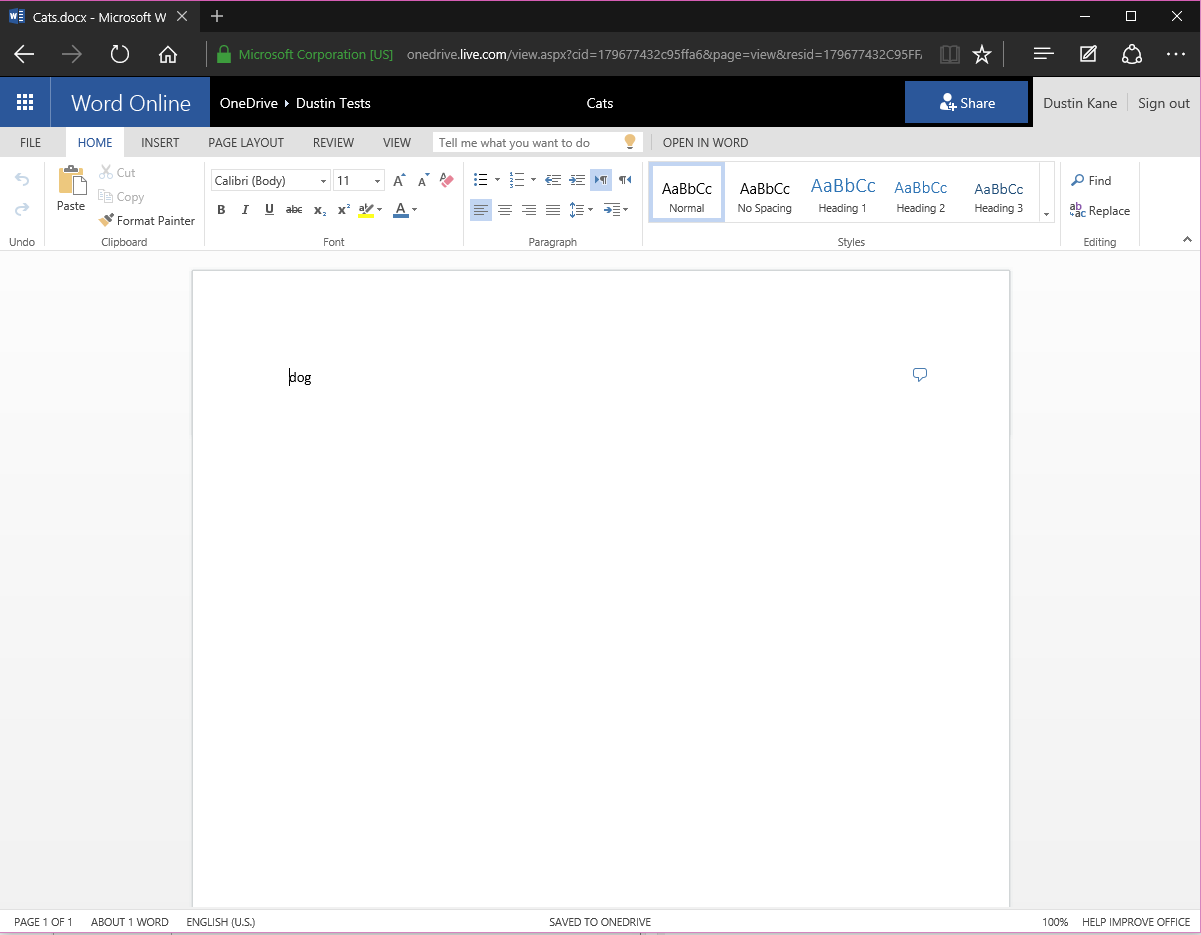
\includegraphics[width=6in]{onedrive}
\caption{OneDrive's ``Word Online'' document editor. Note it is very similar in appearance to Microsoft Word 2013}
\end{figure}

As to Google Drive's success among experienced users, I suspect this is due to Google Drive being slightly more responsive than OneDrive. The first task is incredibly basic and anyone who claims to be experienced in either of these services should know how to do these very easily. At an average difference of 0.6 seconds in Google Drive's favor, I do not think Google Drive has an interface that made this task particularly more efficient. In my experience, however, loading the ``share'' dialog takes a little bit longer in OneDrive, which could explain the difference.

\begin{figure}[h]
\centering
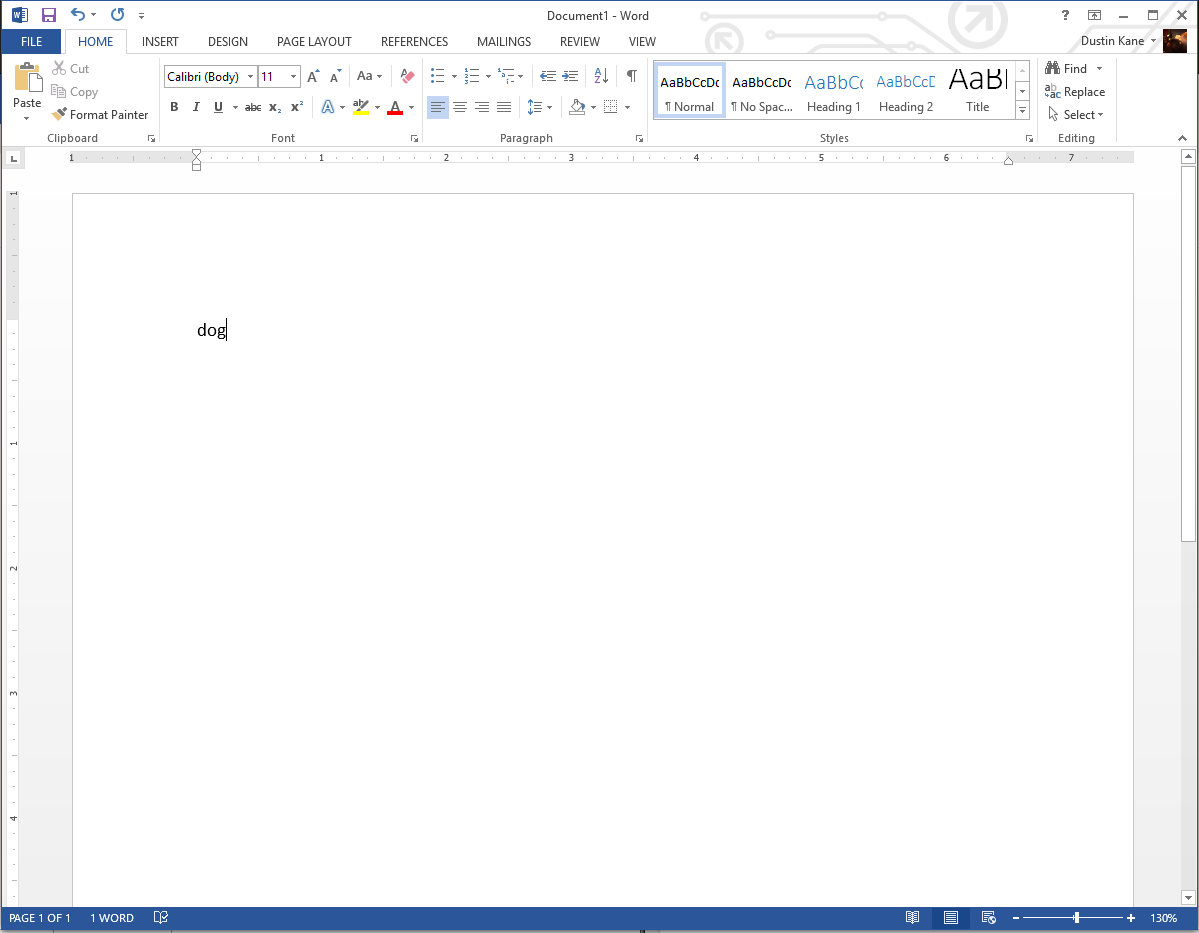
\includegraphics[width=6in]{word}
\caption{Microsoft Word 2013. Note the similarities between this and Figure 1}
\end{figure}

\subsection{The Second Task}

The first task required the user to highlight the word ``dog'' and leave a comment for a collaborator.

For new users, Google Drive was 1.3 seconds faster 

\end{document}